\chapter{T-maps --- užívateľská dokumentácia}
\label{userdoc}
\section{Popis programu T-maps}
Program T-maps načíta mriežkový graf vo forme znakovej matice a vykreslí ho. K danému grafu môže voliteľne načítať dátový súbor, ktorý obsahuje
informácie o~behu algoritmu: informáciu o~navštívených vrcholoch a~o~najkratšej ceste.
Túto maticu aj s~dátami vykreslí na~obrazovku. Výstup pripomína mapu používanú v~počítačových hrách.
Zvláda niekoľko ďalších operácií, ako je priblíženie a~oddialenie mapy, posúvanie sa po~mape a~uloženie aktuálne prehliadaného úseku mapy.


\section{Formát vstupu a výstupu}
Presný formát vstupného súboru s~mriežkovým grafom je popísaný v~\cite{sturtevant2012benchmarks} a~je zhodný s~formátom, 
ktorý používa algoritmus. Znaková matica obsahuje rôzne znaky reprezentujúce rôzne herné prvky.
Strom je reprezentovaný znakom \uv{T}(tree), voda znakom \uv{W}(water), priechodná oblasť(a teda znak, ktorý reprezentuje
vrchol grafu) znakom \uv{.}, prípadne \uv{S} (swamp).

Dátový súbor obsahuje dva riadky. Prvý riadok obsahuje medzerou oddelené čísla vrcholov, ktoré ležia na najkratšej ceste.
Druhý riadok obsahuje čísla vrcholov, ktoré boli navštívené počas behu algoritmu. 
Vrcholy sú popísané jedným číslom tak, ako to bolo popísané v poznámke~\ref{note:popis_vrcholu}.

Výstup môže byť exportovaný do viacerých grafických formátov, medzi ktorými sú GIF, PNG, BMP a JPEG.



\section{Vykreslenie znakovej matice}

Znaky v matici môžu byť vykreslené dvomi spôsobmi. V takzvanom bichromatickom móde sa na vykreslenie matice použijú dve farby.
Svetlejšou farbou sú vykreslené znaky reprezentujúce vrcholy matice (v hrách ide o priechodný terén), tmavšou farbou sú vykreslené znaky, ktoré
nereprezentujú žiaden vrchol. Ide o stromy, vodu a podobne.

Pri plnofarebnom vykreslení sú znaky vykreslené nasledovnými farbami:
\begin{itemize}
\item Strom - zelená.
\item Voda - modrá.
\item Bažina a defaultná priechodná oblast - papájovožltá.
\item Defaultná nepriechodná oblasť - sivá.
\end{itemize}


\section{Vykreslenie dátového súboru}
Pokiaľ bol vrchol prehľadávaný počas hľadania najkratšej cesty, jeho farba bude oranžová. Ak je dokonca súčasťou najkratšej cesty, 
tak bude červený.

\section{Ukážky programu}


Na~obrázkoch nižšie sa~nachádza znaková matica veľmi malého mriežkového
 grafu (Obr.~\ref{fig:testmap_znakova_matica}) a~ukážky z~programu:
 screenshot programu pri načítanej znakovej matici vo~farebnom móde (Obr.~\ref{fig:testmap_program_color}),
 a~screenshot programu aj s~vyznačenou najkratšou cestou 
 a~prehľadanými vrcholmi v bichromatickom móde(Obr.~\ref{fig:testmap_bichromatic_w_path}). 


\begin{figure}[h]
\centering
$$
  \begin{matrix}
    @&@&@&.&.&.&@&@&@&@ \\
    @&T&T&T&.&.&.&.&.&@\\
    T&T&T&T&T&W&W&S&S&.\\
    T&W&W&W&W&W&W&.&.&.\\
    @&@&@&@&@&@&@&@&@&@\\
  \end{matrix}
$$

\caption{Maticová reprezentácia mriežkového grafu}
\label{fig:testmap_znakova_matica}
\end{figure}


\begin{figure}[h]
\centering
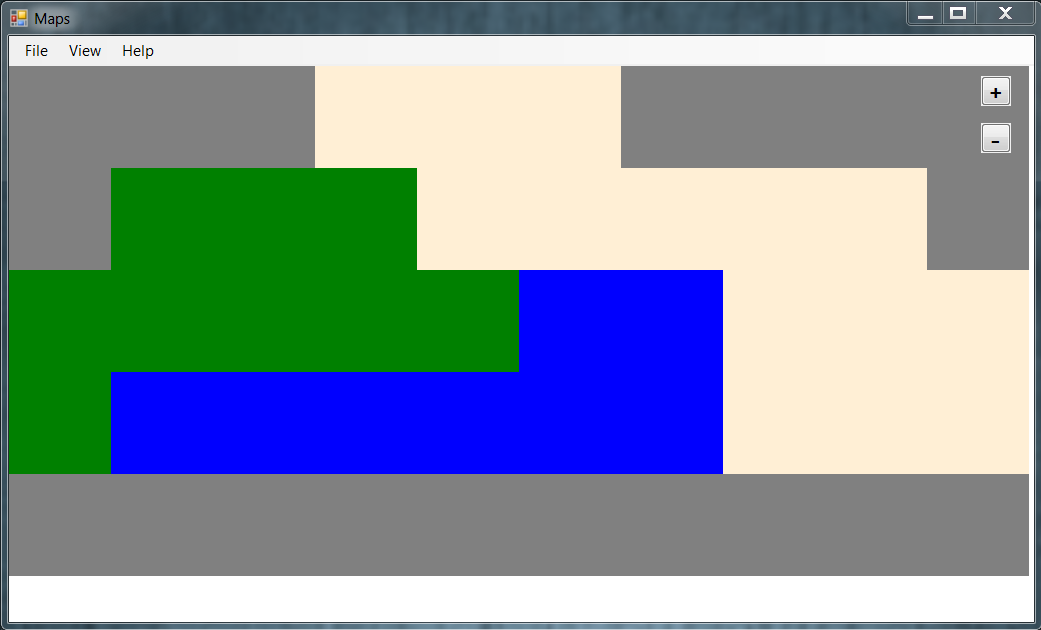
\includegraphics[width=12cm]{./img/testmap_program_color.png}
\caption{Screenshot programu }
\label{fig:testmap_program_color}
\end{figure}

\begin{figure}[h]
\centering
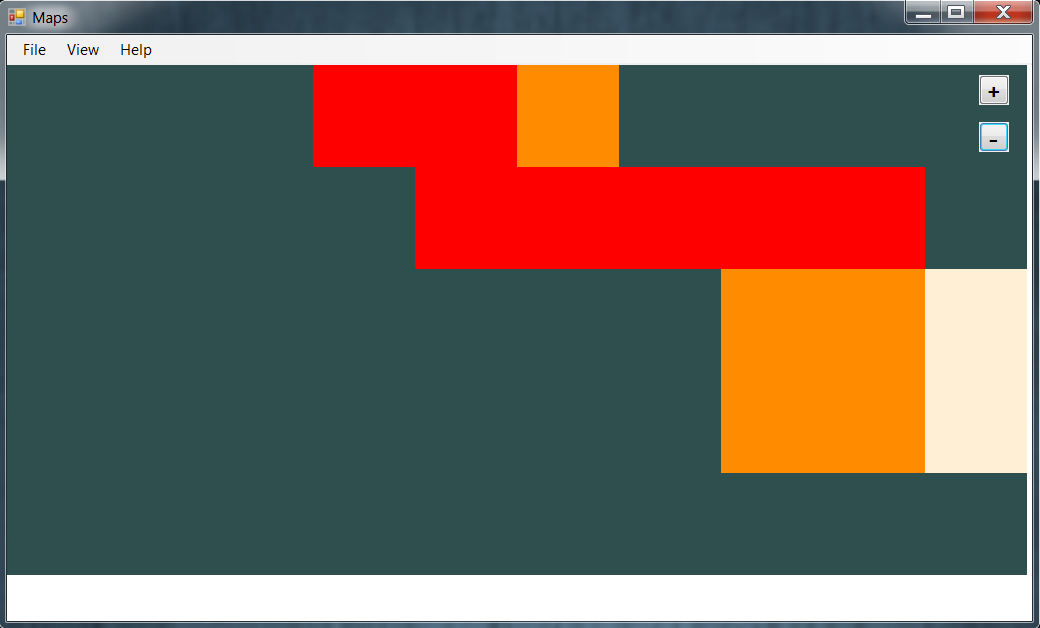
\includegraphics[width=12cm]{./img/testmap_program_bichromatic_w_path.png}
\caption{Vyexportovaný výstup v bichromatickom móde aj s označenou najkratšou cestou a prehľadanými vrcholmi}
\label{fig:testmap_bichromatic_w_path}
\end{figure}
